\label{sec.don_exp}

%L’état initial est préparé selon le protocole décrit en section~\ref{sub_pisih}. Le confinement longitudinal est ensuite supprimé, tandis que le confinement transverse est maintenu, afin d'étudier la dynamique le long de l’axe longitudinal.

%Les profils de densité en bord obtenus pour des temps d’évolution compris entre $\tau = 10$~ms et $\tau = 18$ms sont présentés en Fig.\ref{fig:euler}(a), en fonction de la variable réduite $v = x/\tau$. L’excellent recouvrement des différents profils indique que l’échelle d’Euler est atteinte dans cet intervalle temporel. Au-delà de $\tau = 18$~ms, la dynamique longitudinale ne peut plus être explorée expérimentalement, en raison de la taille finie du gaz initial, préparé dans une configuration semi-homogène.

%Pour des temps d’évolution plus courts, les profils de bord mesurés présentent une forme plus lissée que celle prédite par les équations de GHD à l’échelle d’Euler. Cette différence peut s’expliquer soit par une invalidité de l’approximation d’Euler dans ce régime transitoire, en lien avec de fortes variations de densité, soit par le fait que la coupure initiale à $t = 0$ n’est pas parfaitement abrupte, ce qui confère au bord initial une largeur finie.

%\begin{figure}[!htb]
%\centering
%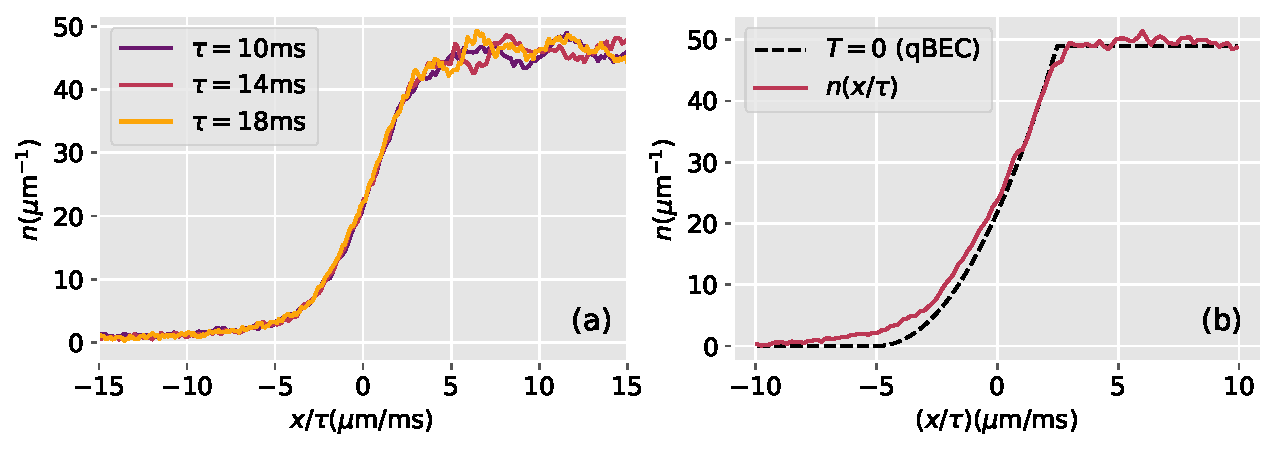
\includegraphics[width=1.0\linewidth]{DWD_GPE_vs_exp_V2.pdf}
%\caption{(a) -- Figure a réfaire -- Profils de densité aux bords obtenus pour différents temps d’évolution $\tau$, représentés en fonction de $x/\tau$ ; (b) Comparaison du profil de bord mesuré avec la prédiction à température nulle issue de la GHD dans le régime quasi-condensat, donnée par l’équation~\eqref{eq:GPE}. Cette dernière constitue une excellente approximation pour la valeur du paramètre d’interaction correspondant aux données, soit $\gamma = 4{,}6 \times 10^{-3}$ (voir Fig.\ref{fig:boundary_profiles_theory}). Le profil de bord présenté en (b) est obtenu après un temps d’expansion de 10ms et provient d’un jeu de données différent de celui de la figure (a).}
%\label{fig:euler}
%\end{figure}
%
%La figure~\ref{fig:euler}(b) présente une comparaison entre le profil de bord mesuré $n(v)$ et la prédiction théorique fondée sur un état initial à température nulle, supposé être l’état fondamental. Pour la valeur du paramètre de Lieb $\gamma = 4{,}6 \times 10^{-3}$, le profil est pratiquement indiscernable de celui obtenu dans le régime de quasi-condensat, justifiant l’utilisation de l’équation~\eqref{eq:GPE} pour la comparaison.

%L’accord entre la prédiction théorique et les données expérimentales est satisfaisant, en particulier dans la région de forte densité. Les écarts observés par rapport à la forme parabolique prédite peuvent être attribués à des effets liés à une entropie non nulle, qui seront analysés dans la section suivante.


%%%%%%
L’état initial est préparé selon le protocole décrit en section~\ref{sub_pisih}. Une fois cet état établi, le confinement longitudinal est supprimé, tandis que le confinement transverse est maintenu, permettant ainsi d'étudier l’expansion du gaz le long de l’axe longitudinal.

Conformément aux prédictions hydrodynamiques à l’échelle d’Euler, la dynamique du système à long temps peut être caractérisée par une forme auto-similaire des profils de densité en bord, de la forme :
\begin{equation}
n(x; t) = n^\ast\left(\frac{x}{t}\right).
\end{equation}
Cette propriété résulte de l’invariance d’échelle des équations de la GHD et se vérifie pour tout système régissant une dynamique eulérienne.

Cette prédiction a été testée expérimentalement en superposant les profils de densité en bord, obtenus à partir d’un même état initial, pour différents temps de déformation $t$, en les représentant en fonction de la variable réduite $v = x/t$. Les profils ainsi mis à l’échelle sont présentés en Fig.~\ref{fig:euler}(a) pour des temps compris entre $t = 10$~ms et $t = 18$~ms. L’excellent recouvrement des courbes confirme que le régime balistique est atteint dans cet intervalle de temps.

%En effet, cette description hydrodynamique à l’échelle d’Euler n’est valide que dans un domaine temporel restreint $\tau \in [\tau_m, \tau_M]$, qui dépend notamment des paramètres du système initial (taille du nuage, température, etc.) :
%\begin{itemize}
%    \item Pour $t > t_M$, la modélisation basée sur une déformation d’un bord semi-infini n’est plus adéquate, car la densité maximale du gaz diminue significativement par rapport à celle de l’état initial. Dans notre cas, on estime $t_M \sim 18$~ms, au-delà duquel les effets de taille finie deviennent non négligeables.
%    \item Pour $t< t_m$, l’accord avec la GHD est également perdu. Trois effets principaux peuvent expliquer cette déviation :
%    \begin{enumerate}
%        \item La coupure initiale induite par la méthode de sélection n’est pas parfaitement abrupte ; elle agit sur une échelle spatiale de l’ordre du micron, ce qui affecte significativement la dynamique à très court terme.
%        \item La résolution optique du système d’imagerie (supérieure à 1~µm) limite la capacité à résoudre la structure du bord pour des temps d’expansion trop courts.
%        \item Les équations de la GHD ne sont valides que dans la limite des grandes échelles spatio-temporelles, ce qui rend leur application inappropriée pour modéliser des évolutions inférieures à $t_m = 6 \pm 2$~ms.
%    \end{enumerate}
%\end{itemize}

En effet, cette description hydrodynamique à l’échelle d’Euler n’est valable que dans un domaine temporel restreint $t\in [t_m, t_M]$, qui dépend notamment des paramètres initiaux du système, tels que la taille du nuage ou la température. Pour des temps $\tau > t_M$, estimés autour de 18ms dans notre cas, la modélisation fondée sur une déformation d’un bord semi-infini devient inadaptée, la densité maximale du gaz ayant diminué de manière significative, ce qui rend les effets de taille finie non négligeables. Inversement, pour des temps $t < t_m$, l’accord avec la GHD se détériore également, ce qui peut s’expliquer par le caractère non parfaitement abrupt de la coupure initiale — effective sur une échelle de l’ordre du micron —, par la résolution limitée du système d’imagerie (supérieure à 1~$\mu$m) qui empêche de distinguer les détails du bord à très court terme, et enfin par la nature même des équations de la GHD, qui ne sont rigoureusement valables que dans la limite des grandes échelles spatio-temporelles ; dans nos conditions expérimentales, on estime cette borne inférieure à $t_m = 6 \pm 2$~ms.

%La Fig.~\ref{fig:euler}(b) illustre la comparaison entre un profil de bord mesuré à $\tau = 10$~ms et la prédiction théorique obtenue à température nulle dans le régime de quasi-condensat, donnée par l’équation~\eqref{eq:GPE}. Pour la valeur du paramètre de Lieb $\gamma = 4{,}6 \times 10^{-3}$, la solution GHD est quasiment indiscernable de celle du régime de quasi-condensat, ce qui valide l’utilisation de ce dernier pour la comparaison. L’accord est particulièrement bon dans la région de haute densité ; des écarts apparaissent néanmoins en bord, potentiellement attribuables à une entropie initiale non nulle, dont l’effet sera discuté dans la section suivante.

\begin{figure}[!htb]
\centering
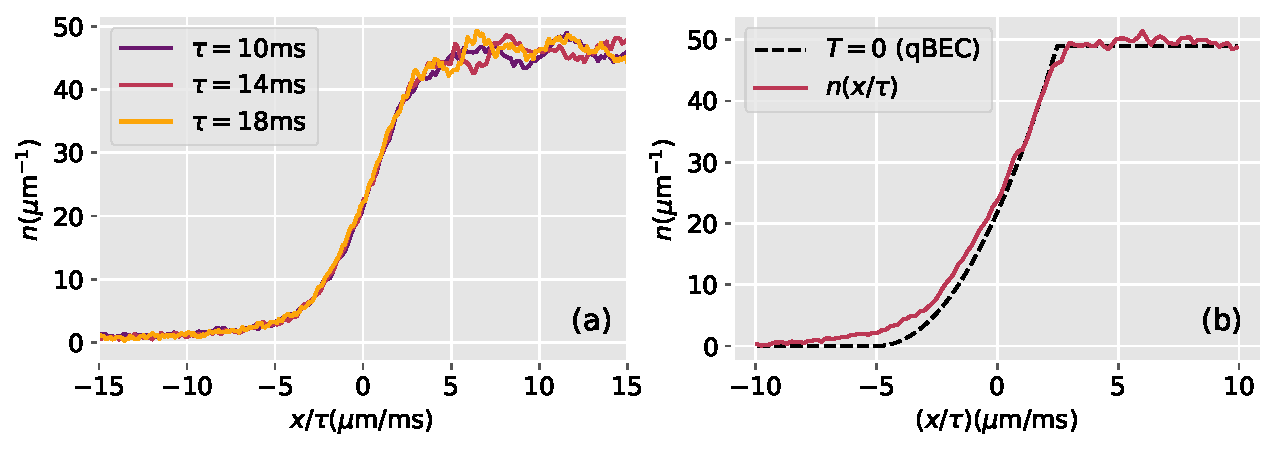
\includegraphics[width=1.0\linewidth]{DWD_GPE_vs_exp_V2.pdf}
\caption{(a) Profils de densité aux bords obtenus pour différents temps de déformation $t$, représentés en fonction de la variable réduite $x/t$. Le bon recouvrement des profils témoigne d’une dynamique balistique conforme à la GHD à l’échelle d’Euler. (b) Comparaison d’un profil mesuré à $t = 10$~ms avec la prédiction à température nulle de la GHD dans le régime de quasi-condensat (équation~\eqref{eq:GPE}), pour un paramètre de Lieb $\gamma = 4{,}6 \times 10^{-3}$.}% Les données de (b) proviennent d’un jeu expérimental distinct de celui de (a).}
\label{fig:euler}
\end{figure}

